\documentclass[t,aspectratio=1610]{beamer}

\usepackage{listings}
\usepackage{graphicx}
\usepackage{tikz}
\usepackage{xcolor}

\newcommand{\lp}{\left(}
\newcommand{\rp}{\right)}

\usetheme{default}
\beamertemplatenavigationsymbolsempty\setbeamersize{
	text margin left=0.75cm,
	text margin right=0.75cm
}

% Title
\setbeamerfont{title}{size=\LARGE, 
					  series=\bfseries,
					  family=\rmfamily}
\setbeamercolor{title}{fg=black}
\setbeamertemplate{frametitle}{
	\nointerlineskip\;
	\begin{beamercolorbox}[sep=.1ex,
						   wd=\paperwidth,
						   leftskip=0.5cm,
						   rightskip=0pt]{frametitle}
		\usebeamerfont{frametitle}
		\usebeamercolor[fg]{frametitle}
		\\
		\hfill
		\insertframetitle\;
		\strut\;
	\end{beamercolorbox}
}
% Alerted text
\setbeamerfont{alerted text}{series=\bfseries}
\setbeamercolor{alerted text}{fg=black}
% Itemize
\setbeamercolor{frametitle}{fg=black}
\setbeamercolor{itemize item}{fg=black}
\setbeamercolor{itemize subitem}{fg=black}
\setbeamercolor{itemize subsubitem}{fg=black}
\setbeamertemplate{itemize item}[circle]
\setbeamertemplate{itemize subitem}[triangle]
% Enumerate
\setbeamercolor{enumerate item}{fg=black}
\setbeamercolor{enumerate subitem}{fg=black}
% Blocks
\setbeamercolor{block body example}{fg=black!90,
									bg=black!10}
\setbeamercolor{block title example}{fg=white,
									 bg=black!30}
\setbeamertemplate{blocks}[shadow=true]

\title{Bachelor Project SP 2021 $ \cdot $ Demo 2}
\subtitle{Expression Generator}
\author{Bevilacqua Joey}
\institute{Universit\`a della Svizzera Italiana}
\date{May 5, 2021}

\begin{document}

% Slide 1
\begin{frame}
\maketitle
\end{frame}

% Slide 2.0
\begin{frame}
\frametitle{Project objective}
\begin{itemize}
\item The computer generates some code
\end{itemize}
\end{frame}

% Slide 2.1
\begin{frame}
\frametitle{Project objective}
\begin{itemize}
\item The computer generates some code
	  \begin{enumerate}
	  \item Language grammar
			\begin{itemize}
			\item Math grammar
			\item JSON grammar
			\item BSL (Racket) grammar
			\item Java grammar
			\item $ \dots $
			\end{itemize}
	  \end{enumerate}
\end{itemize}
\end{frame}

% Slide 2.2
\begin{frame}
\frametitle{Grammar}
\begin{center}
	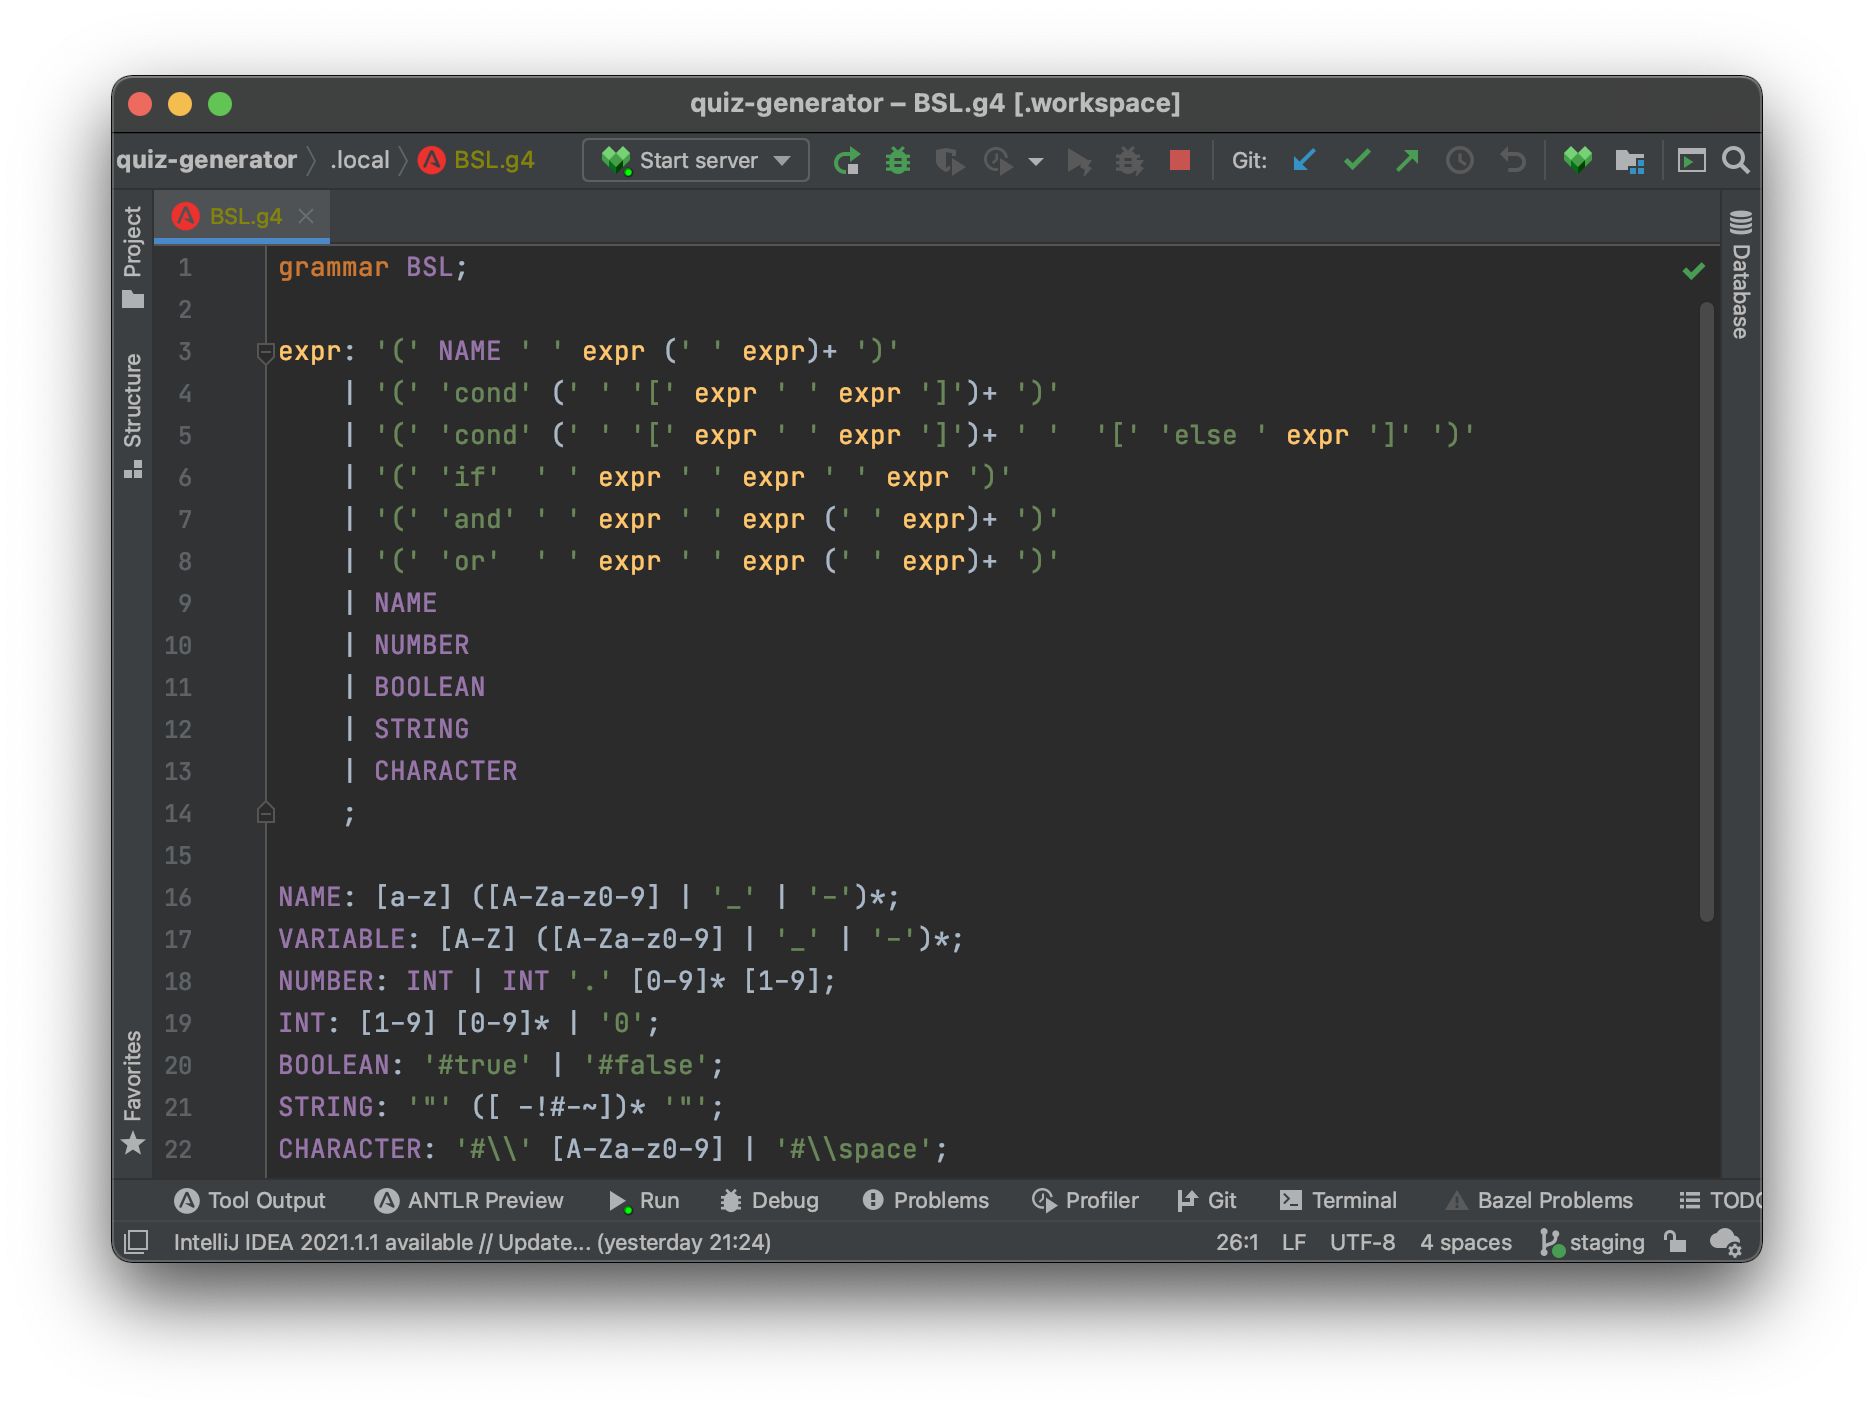
\includegraphics[width=0.7\textwidth]{img/grammar_bsl} \\
	{(A subset of) the BSL Racket language grammar}
\end{center}
\end{frame}

% Slide 2.3
\begin{frame}
\frametitle{Project objective}
\begin{itemize}
\item The computer generates some code
	  \begin{enumerate}
	  \item Language grammar
			\begin{itemize}
			\item Math grammar
			\item JSON grammar
			\item BSL (Racket) grammar
			\item Java grammar
			\item $ \dots $
			\end{itemize}
	  \item Constraints
			\begin{itemize}
			\item Starting rule
			\item Rule inclusion
			\item Expression tree depth
			\end{itemize}
	  \end{enumerate}
\end{itemize}
\end{frame}

% Slide 2.4
\begin{frame}
\frametitle{Project objective}
\begin{itemize}
\item The computer generates some code
	  \begin{enumerate}
	  \item Language grammar
			\begin{itemize}
			\item Math grammar
			\item JSON grammar
			\item BSL (Racket) grammar
			\item Java grammar
			\item $ \dots $
			\end{itemize}
	  \item Constraints
			\begin{itemize}
			\item Starting rule
			\item Rule inclusion
			\item Expression tree depth
			\end{itemize}
	  \item Interfaces
			\begin{itemize}
			\item Command line
			\item Web (Expression Tutor)
			\end{itemize}
	  \end{enumerate}
\end{itemize}
\end{frame}

% Slide 3.0
\begin{frame}
\frametitle{Let's generate something!}
Let's generate an expression using a simple math grammar
($ + $, $ - $, $ \times $ and $ \div $).\\
We want its expression tree to have depth 5. \medbreak
Something like
$ \lp \lp 45 + 81.3 \rp \times \lp \lp 6536 \div 1.9 \rp - 10.3 \rp \rp + 3.14 $: \\
\begin{center}
	\includegraphics[width=0.48\textwidth]{img/trees_expectation}
\end{center}
\end{frame}

% Slide 3.1
\begin{frame}
\frametitle{Let's generate something!}
Let's run our expression generator:
\begin{center}
	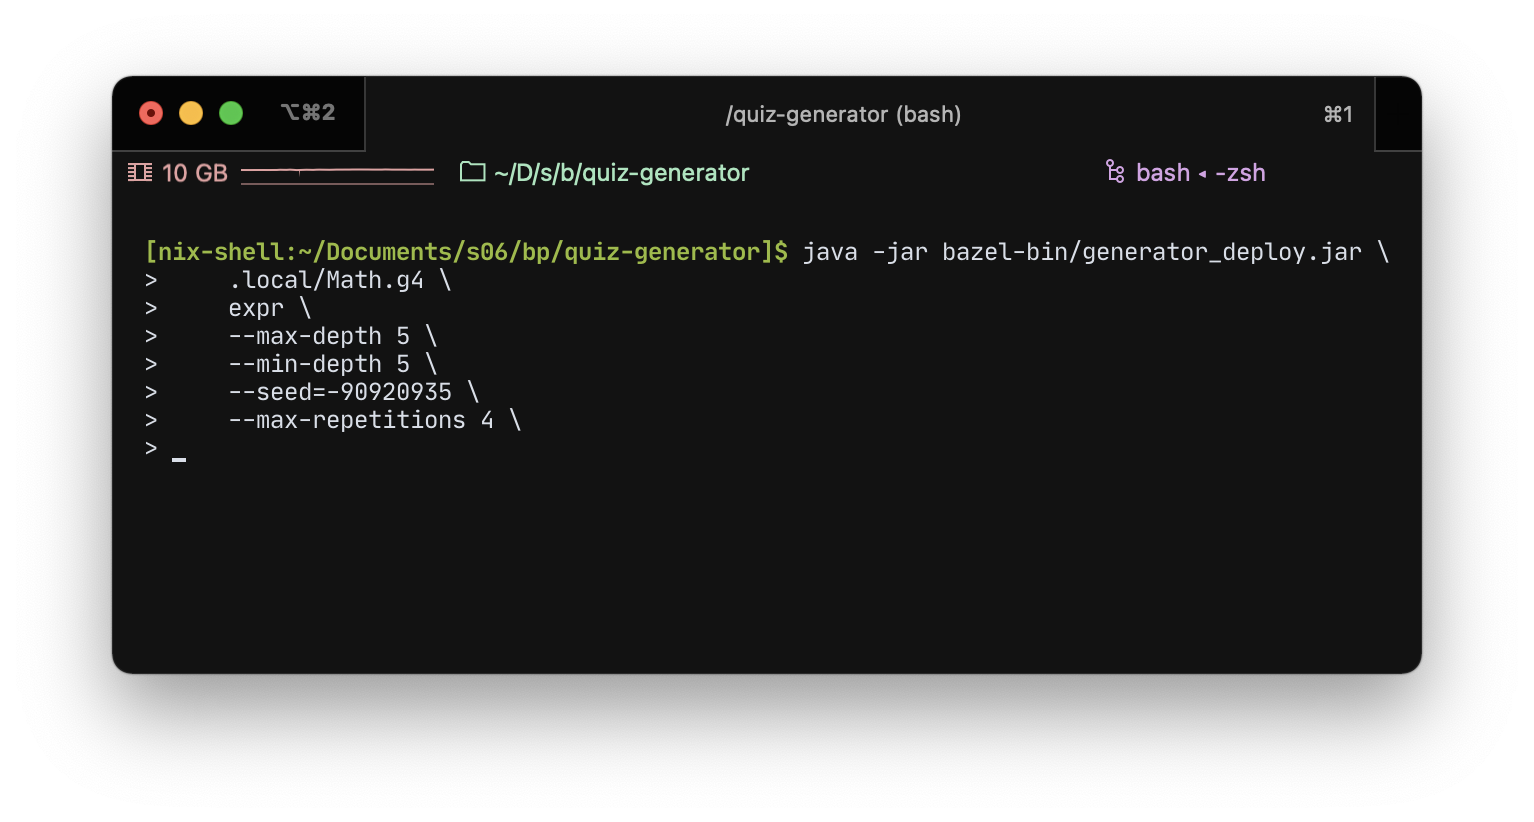
\includegraphics[width=0.8\textwidth]{img/trees_example_0}	
\end{center}
\end{frame}

% Slide 3.2
\begin{frame}
\frametitle{Let's generate something!}
And we get ``$ 6536 / 1.9 $'' \dots?
\begin{center}
	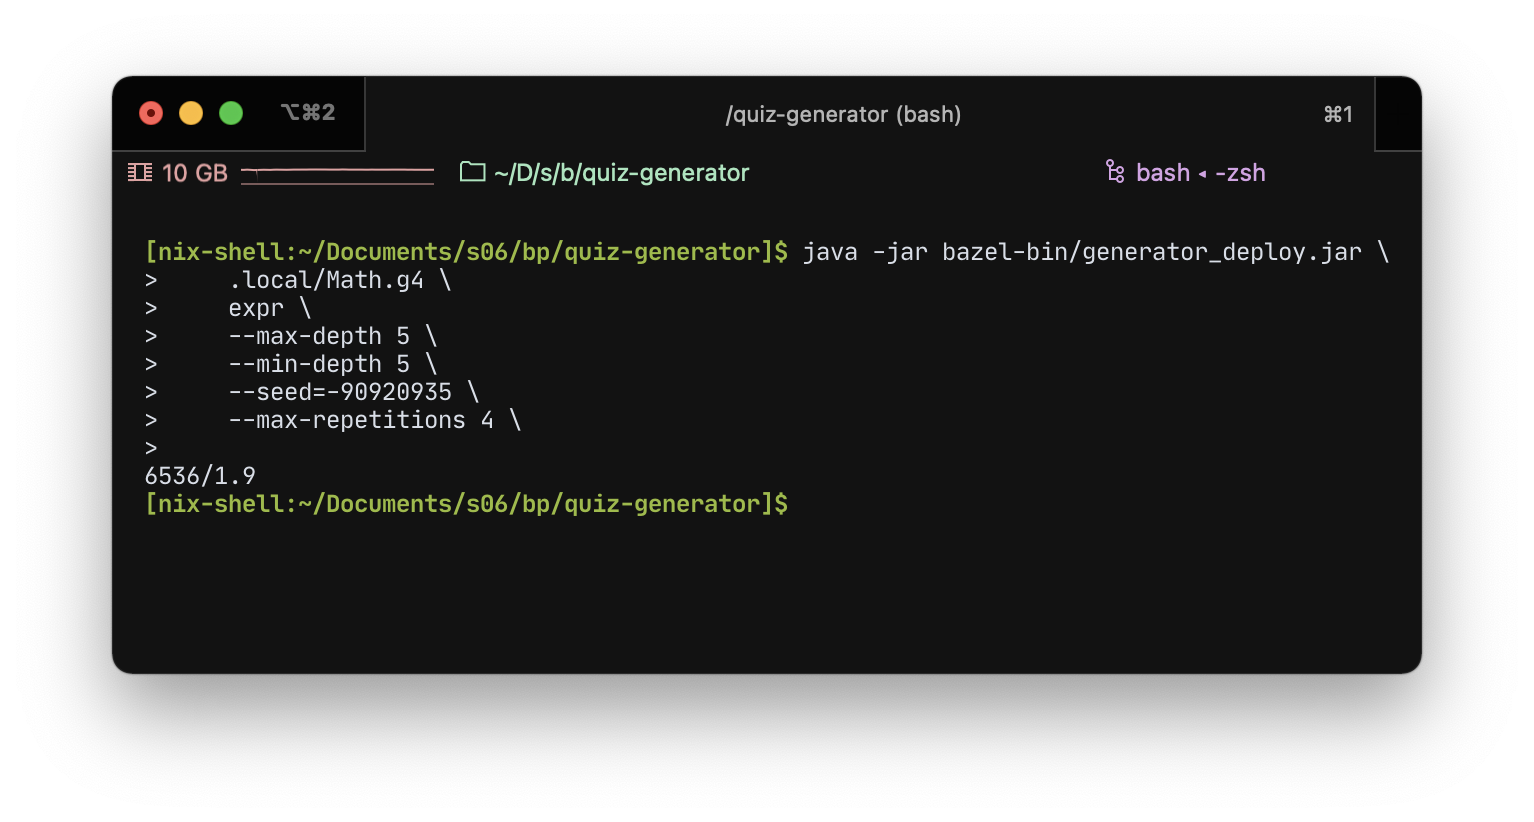
\includegraphics[width=0.8\textwidth]{img/trees_example_1}	
\end{center}
\end{frame}

% Slide 3.3
\begin{frame}
\frametitle{Let's generate something!}
This is how we'd represent the generated expression:
\begin{center}
	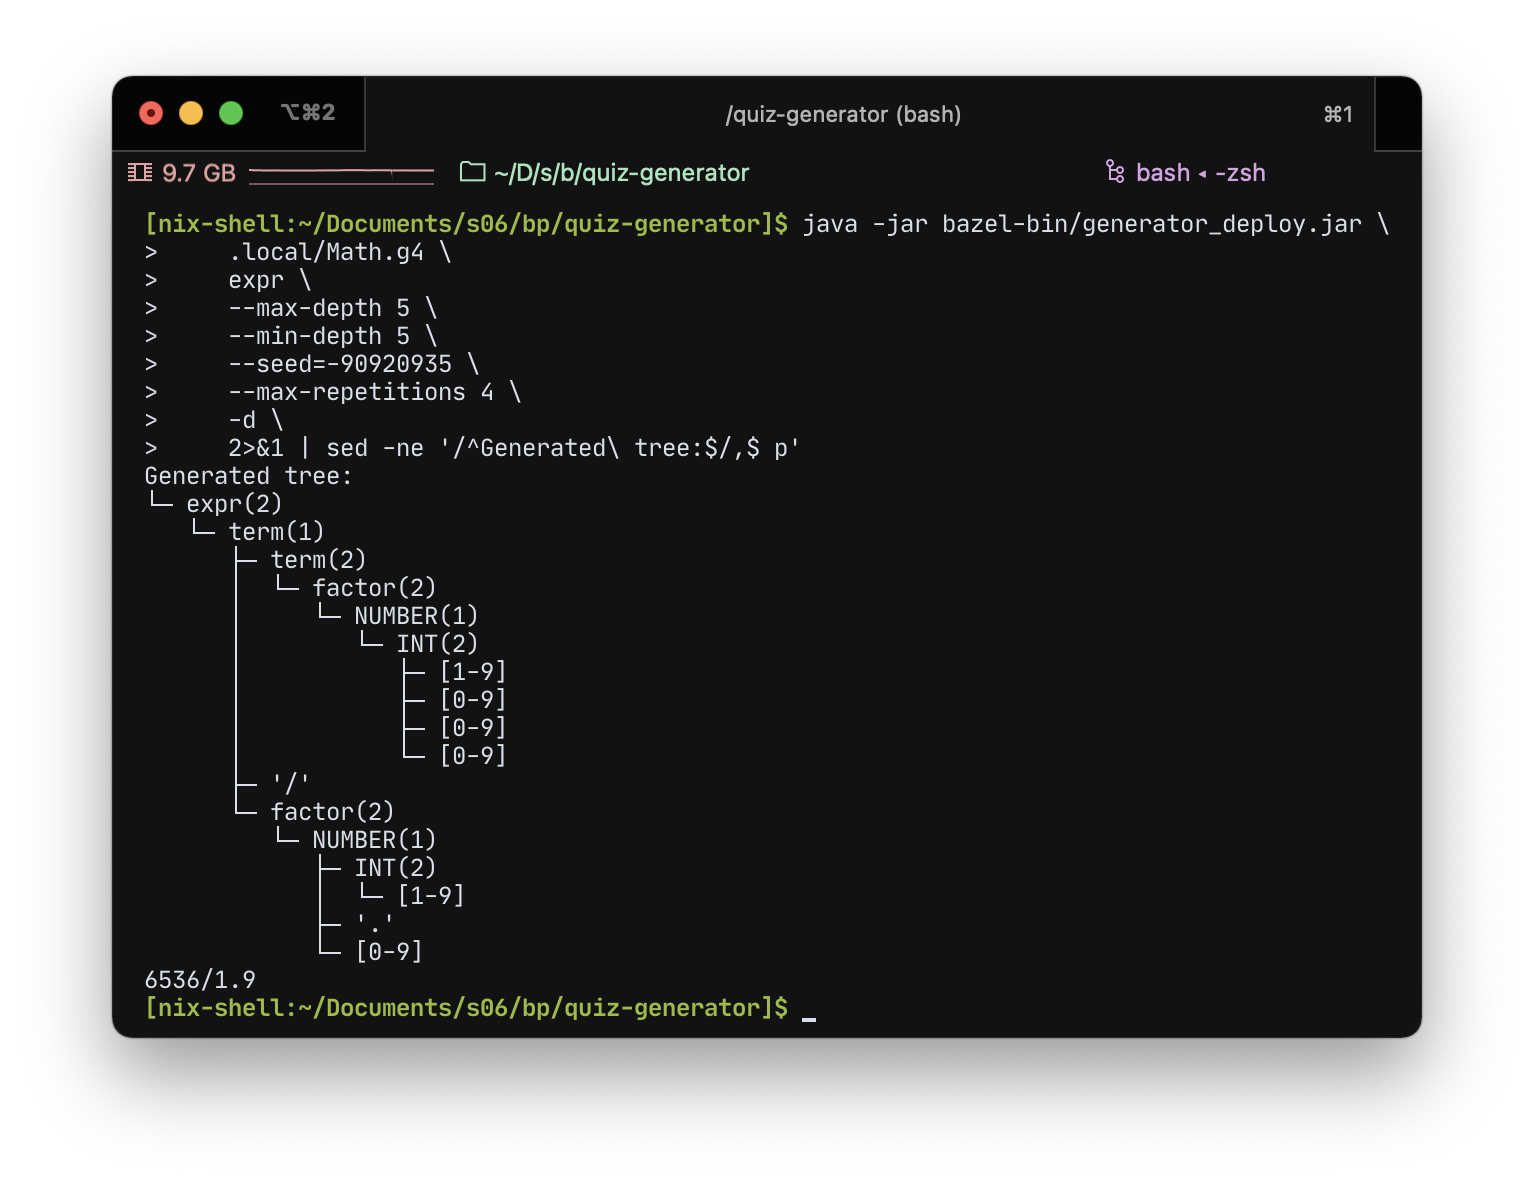
\includegraphics[width=0.4\textwidth]{img/trees_concrete}
\end{center}
It's clear that this tree doesn't have depth 5. \\
\textit{This expression generator thing is so bad it can't even count up to 5.}
\end{frame}

% Slide 3.4
\begin{frame}
\frametitle{Let's generate something!}
If we look at what the program is actually building, we see that the
tree that generated ``$ 6539 / 1.9 $'' has depth $ 6 $
\footnote{
	Due to the grammar and the starting rule, it's not possible
	to have tree depth exactly 5.
} !
\begin{center}
	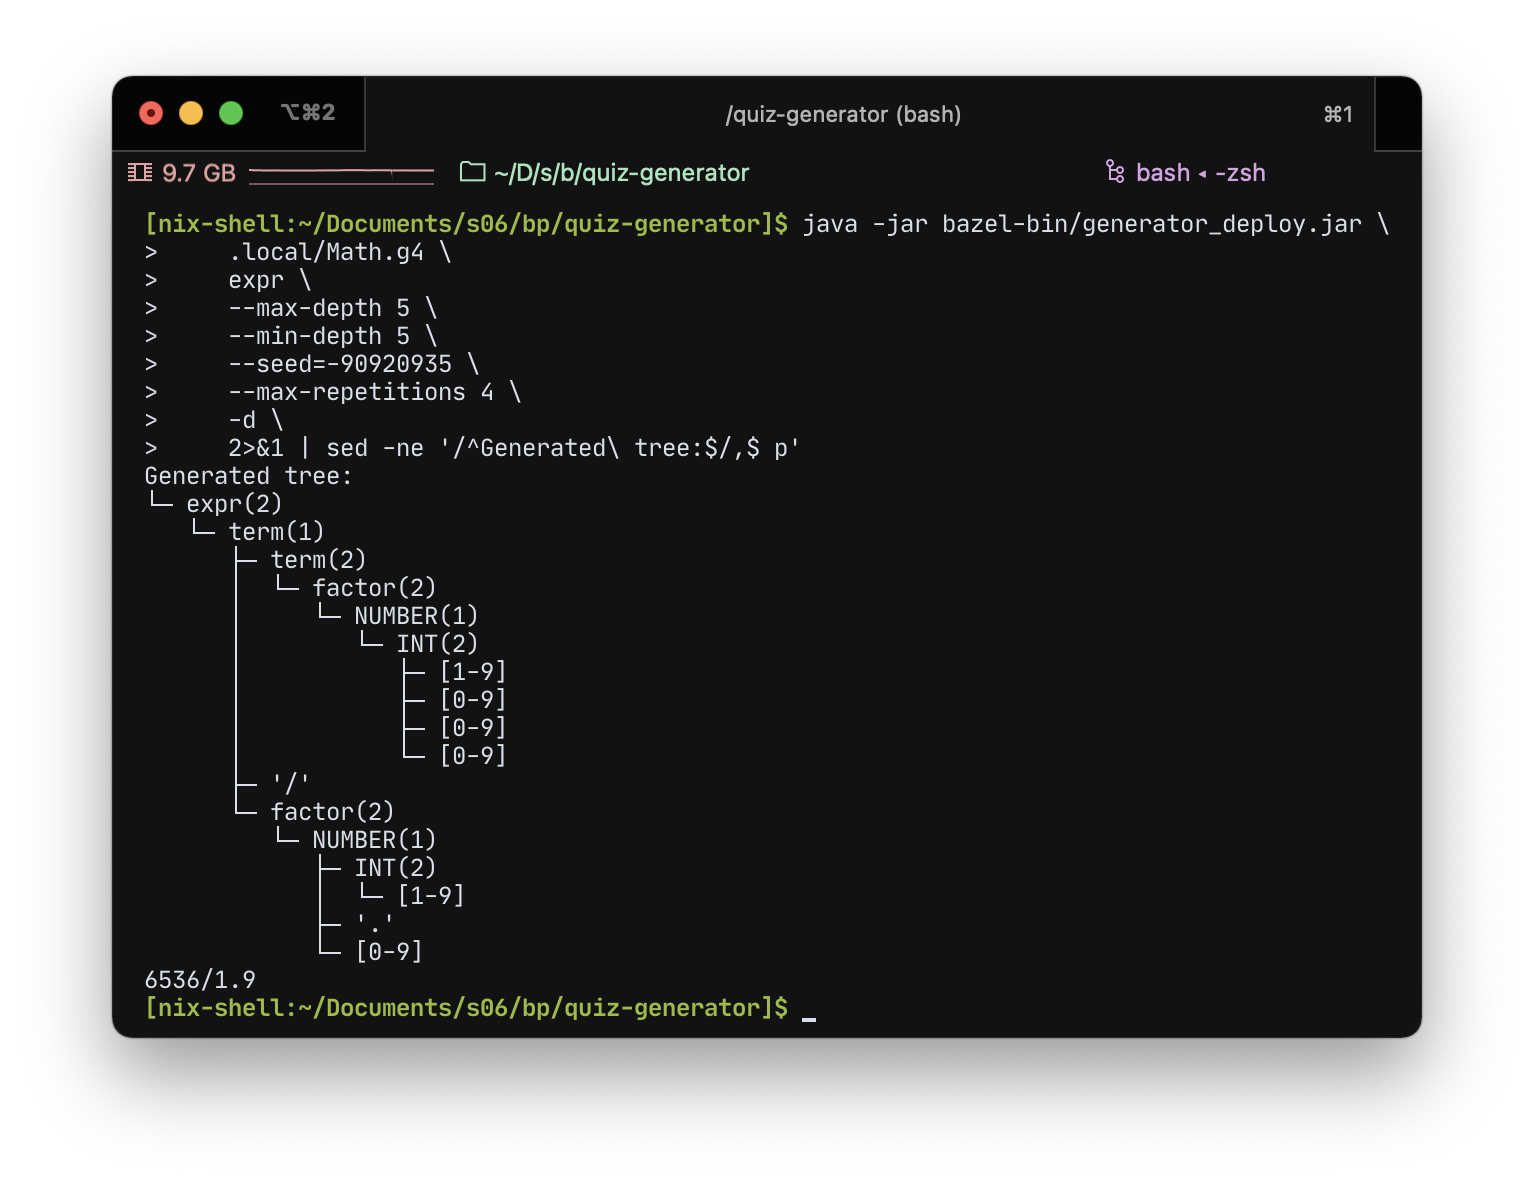
\includegraphics[width=0.6\textwidth]{img/trees_abstract} \\
\end{center}
\end{frame}

% Slide 3.5
\begin{frame}
\frametitle{Trees and trees}
\begin{itemize}
\item What we usually represent in expression tutor is the
	  \textbf{concrete tree}.
\item When we generate expressions from grammars we have to work with
	  \textbf{abstract trees}.
\item We've seen how the abstract tree of an expression does not correspond
	  to the concrete tree of the same expression.
\item The differences between the two depend on how the grammar rules are
	  defined.
\end{itemize}
\end{frame}

% Slide 4.0
\begin{frame}
\frametitle{Command line interface}
\begin{center}
	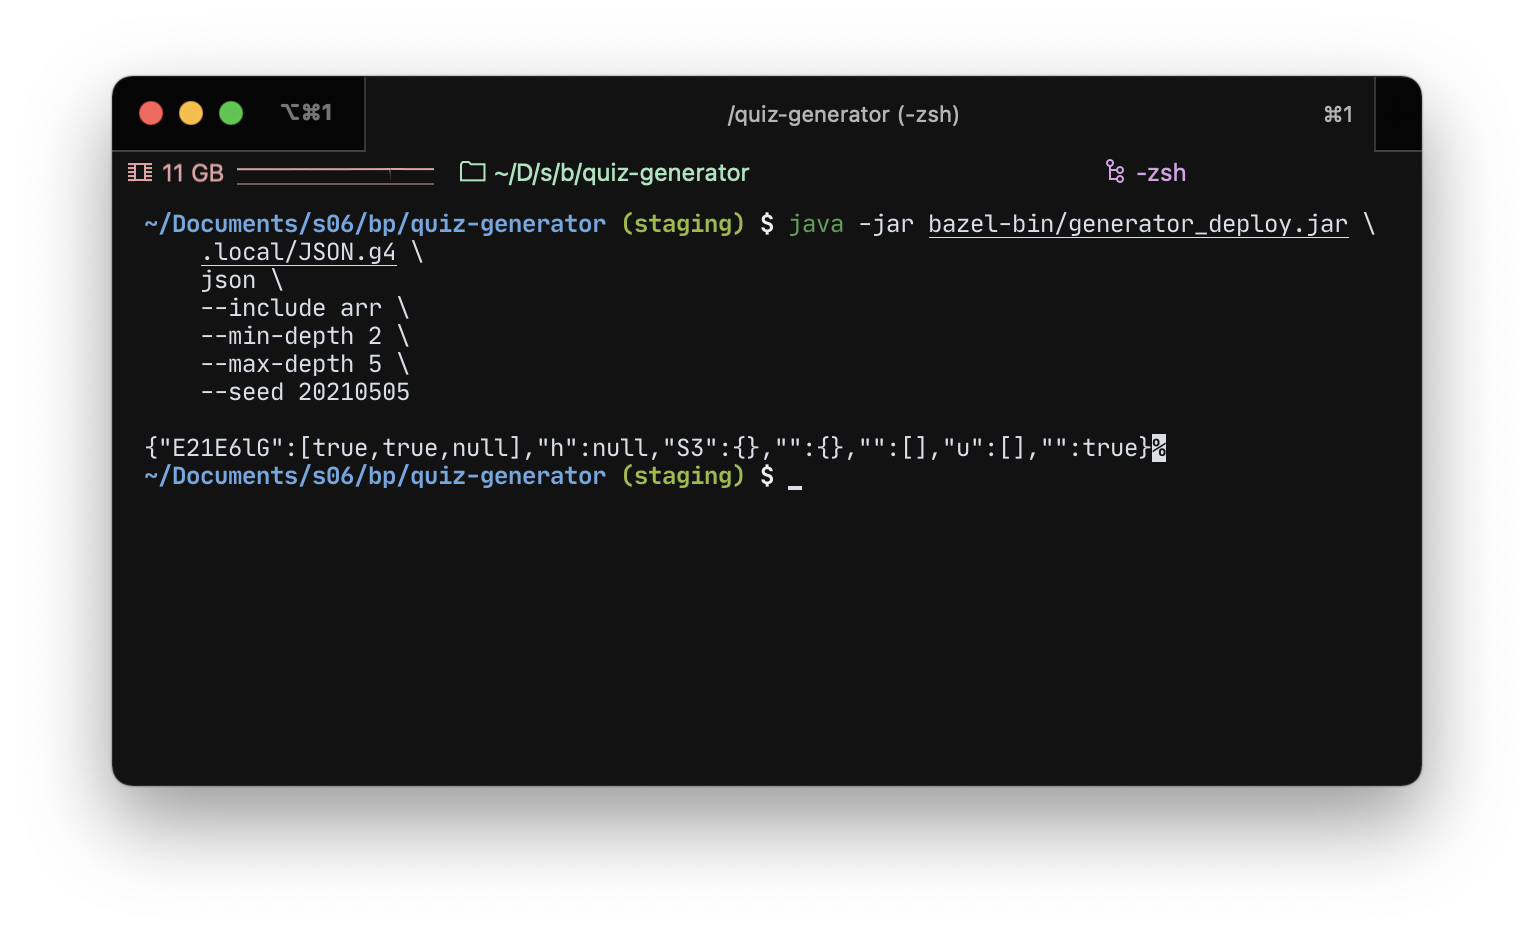
\includegraphics[width=0.8\textwidth]{img/cli} \\
	{Generate a JSON from the command line}
\end{center}
\end{frame}

% Slide 4.1
\begin{frame}
\frametitle{Web interface}
\begin{center}
	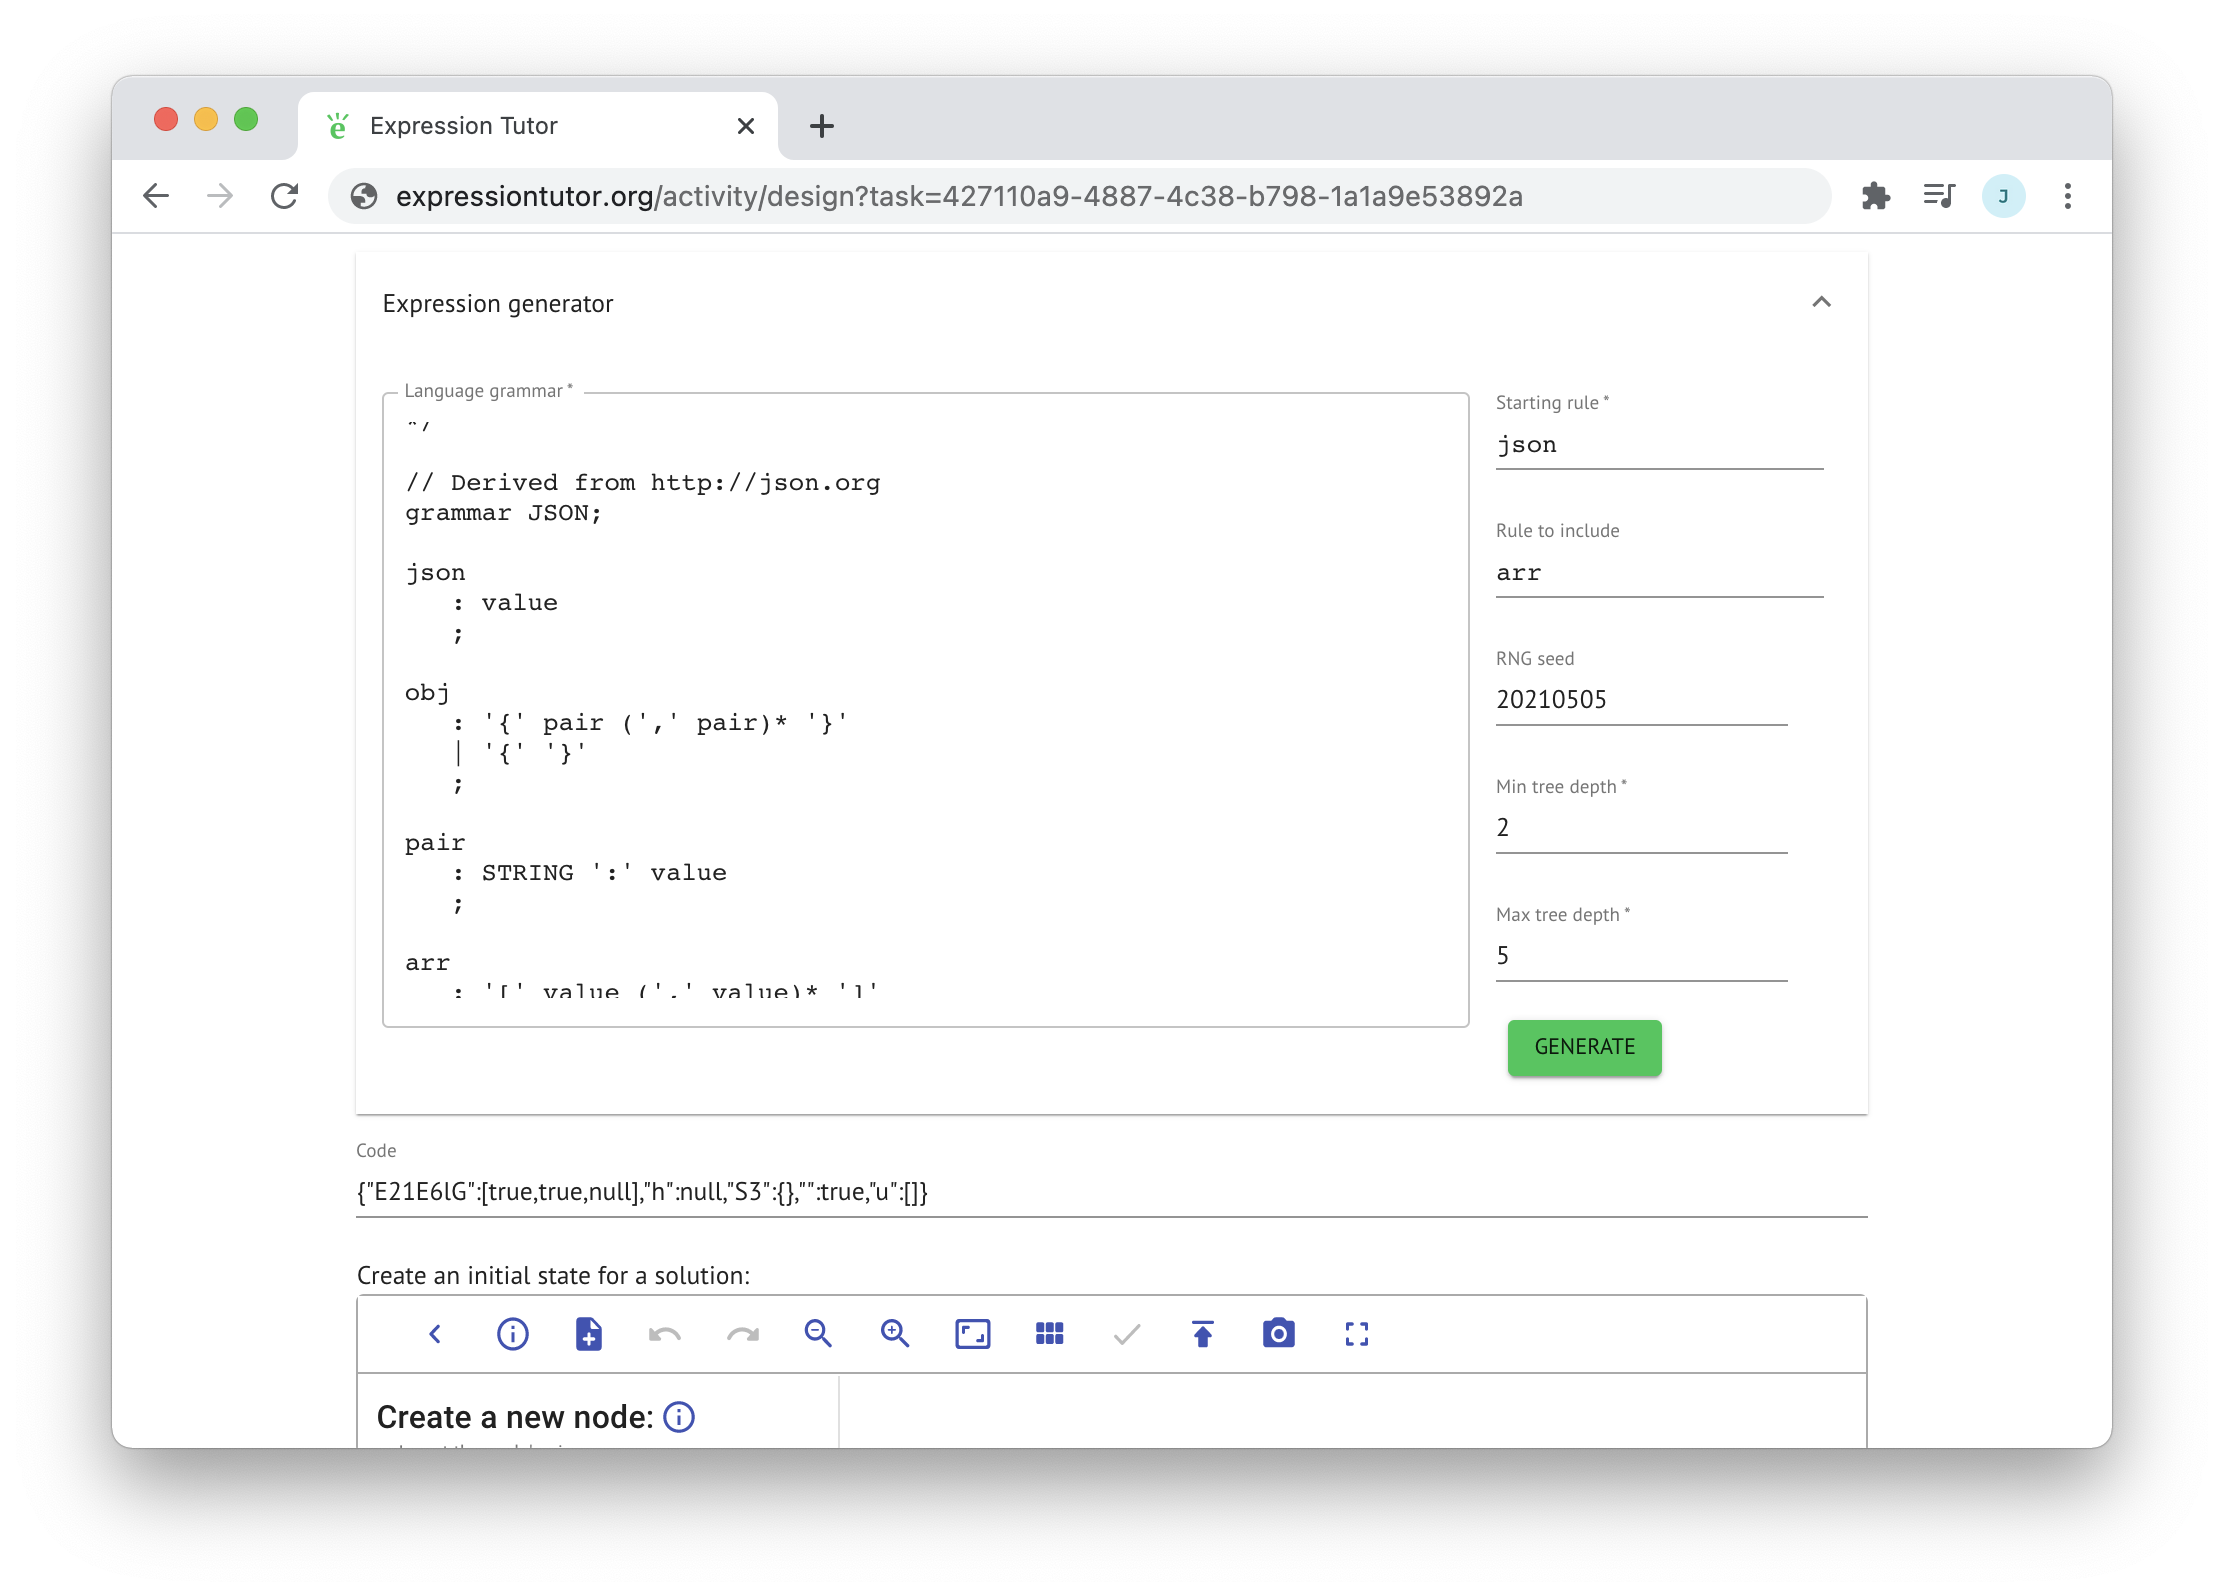
\includegraphics[width=0.7\textwidth]{img/web} \\
	{Generate a JSON from the Expression Tutor activity design}
\end{center}
\end{frame}

% Slide 5.0
\begin{frame}[c]{ }
\centering
\Huge Demo
\end{frame}

\end{document}